\chapter{OpenOCD}
% TODO: referenz openocd doku
% \ref{bib:OpenOCDDoku}
% TODO: CLI beschreiben / putty
% OpenOCD ist ein ''On-Chip Debugger''.\cite{bib:OpenOCDHome}
% Diese Bezeichnung ist allerdings etwas irreführend.
% TODO: Debugger früher erklären (Urs)
% TODO: FT2232 erklären (Urs)
OpenOCD\footnote{http://openocd.org/about/} bildet den Software-Teil eines Debuggers.
Zusammen mit einem Hardware-Adapter bildet OpenOCD einen vollständigen Debugger und kann als Ersatz für einen teuren Debugger, wie beispielsweise dem BDI3000 von Abatron, verwendet werden.

Der Adapter bildet dabei das elektrische Interface zum Prozessor und muss auch auf den Prozessor abgestimmt sein.
Relevant sind dabei unter anderem der Transport Layer (JTAG/SWD), das elektrische Potential und natürlich auch der physikalische Stecker.
In vielen Fällen basieren solche Adapter, wenn sie zusammen mit OpenOCD verwendet werden, auf dem FT2232-Chip von FTDI.
Solch ein generischer Adapter ist in der Abbildung \ref{fig:GenerischerFT2232Adapter} zu sehen.

\begin{figure}[htbp]
	\centering
		% 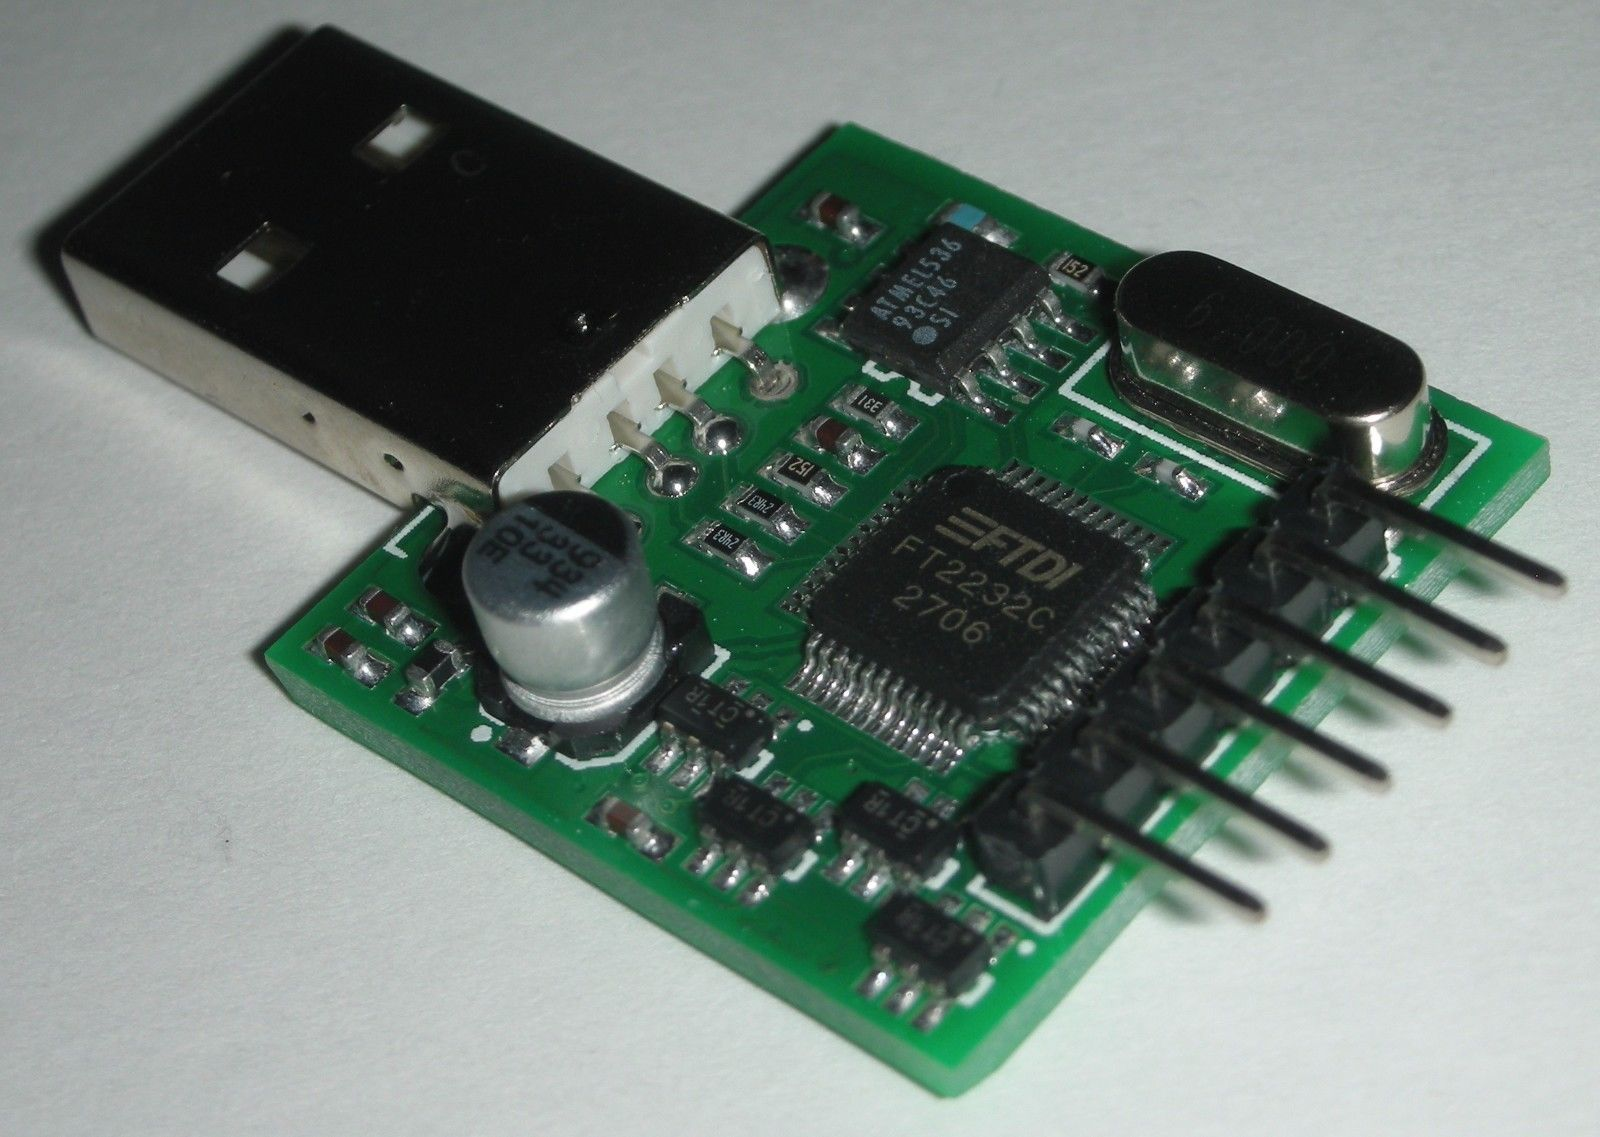
\includegraphics[width=\textwidth,height=\textheight,keepaspectratio]{images/JTAGAdapter.jpg}
		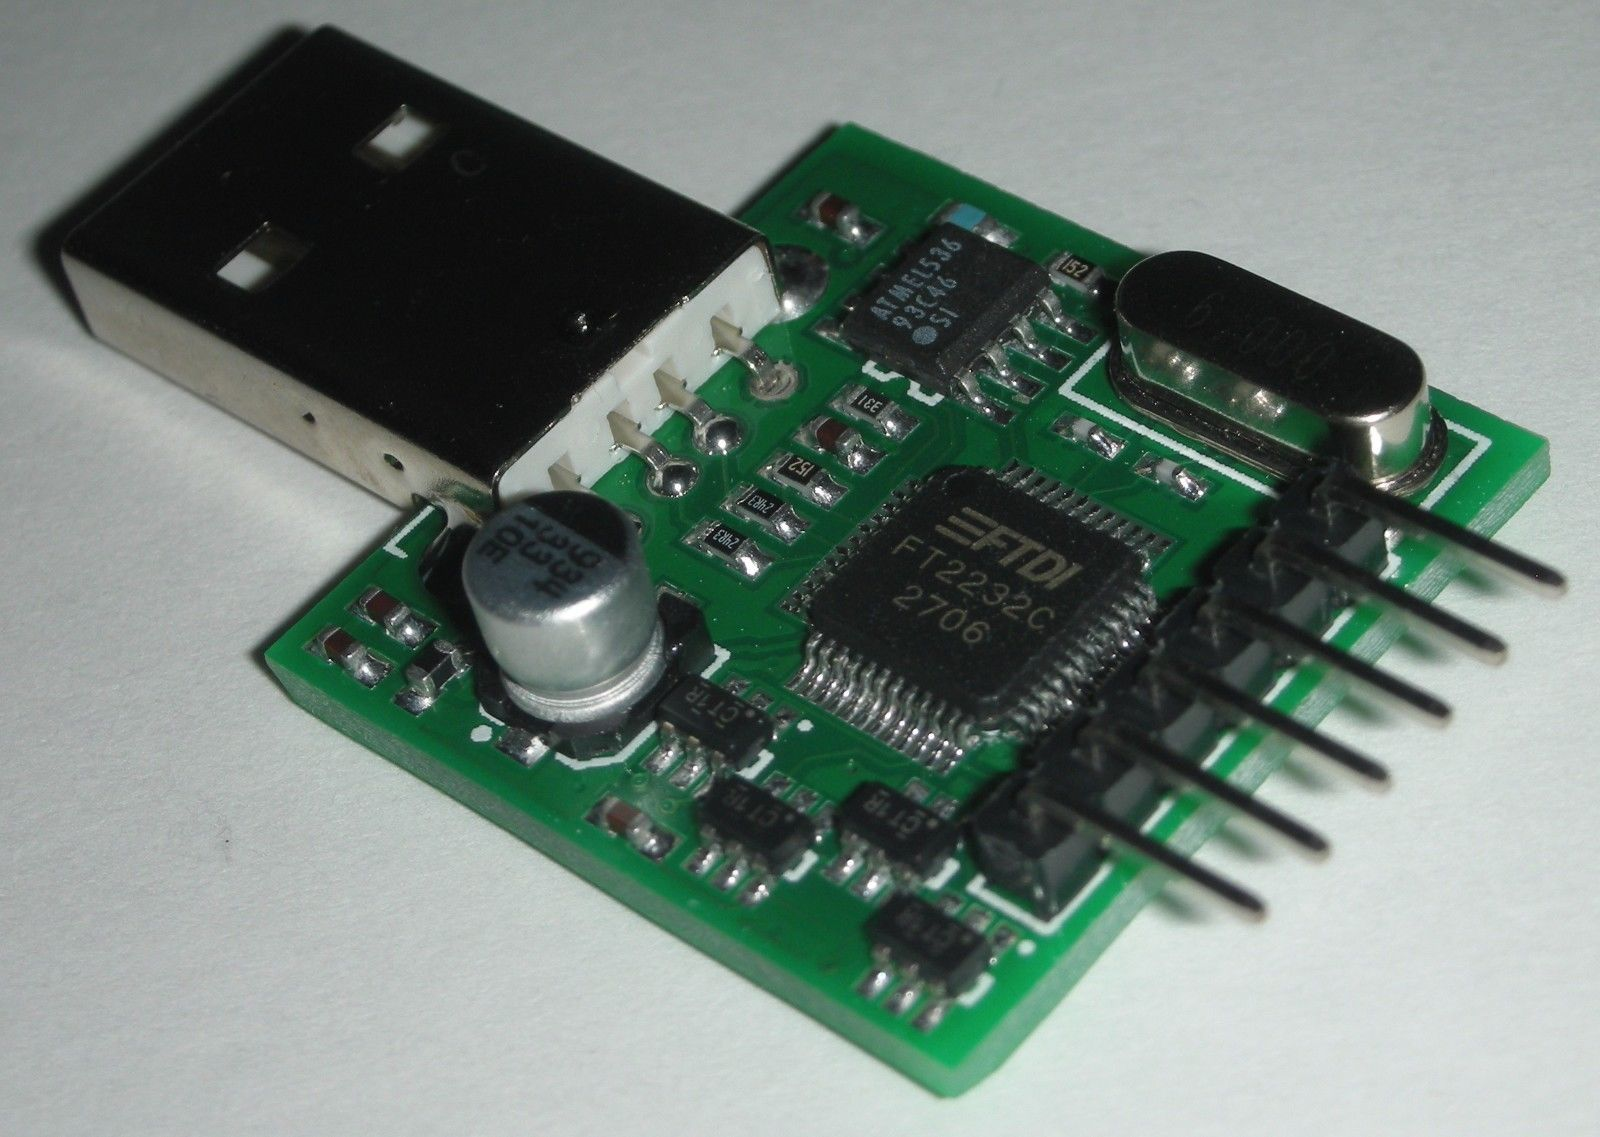
\includegraphics[width=7cm,keepaspectratio]{images/JTAGAdapter.jpg}
	\caption[Generischer JTAG Adapter mit einem FTDI FT2232]{Generischer JTAG Adapter mit einem FTDI FT2232\footnotemark}
	\label{fig:GenerischerFT2232Adapter}
\end{figure}
\footnotetext{https://www.ebay.com/itm/FPU1-FTDI-FT2232-USB-JTAG-XILINX-FPGA-CPLD-programmer-cable-/181635528314 Seite 5}

Bei Experimentierboards ist der FT2232 oft auch direkt auf das Board aufgelötet.
So kann eine einfache USB-Verbindung genutzt werden, um den Prozessor zu debuggen.
Beim Zybo wurde ebenfalls dieser Ansatz verfolgt.
Aus diesem Grund reicht ein einfaches USB Kabel um den Prozessor des Zybos auf einer Hardwareebene debuggen zu können.



\section{Softwareinstallation der OpenOCD-Toolchain}
\label{kapitel:SoftwareinstallationOpenOCDToolchain}
Um OpenOCD nutzen zu können, muss auch der richtige USB-Treiber installiert sein.
In den folgenden Kapiteln wird erklärt, wie der Treiber und auch OpenOCD-Software installiert werden kann.


\subsection{Softwareinstallation - OpenOCD}
OpenOCD kann direkt aus dem Sourcecode kompiliert werden\footnote{http://sourceforge.net/p/openocd/code/} oder es können vorkompilierte Binaries verwendet werden.
Für diese Arbeit wurde das vorkompilierte Windows Binaries\footnote{http://www.freddiechopin.info/en/download/category/4-openocd?download=154\%3Aopenocd-0.10.0} für ARM-Cores mit der Version 0.10.0 verwendet.

Das eigentliche Binary befindet sich im Ordner:\\
\texttt{/openocd-0.10.0/bin-x64/} 

Das Open OCD User Manual\cite{bib:OpenOCDDoku} befindet sich im Ordner:\\
\texttt{/openocd-0.10.0/} 


\subsection{Softwareinstallation - USB-Driver WinUSB}
\label{kapitel:usbTreiber}
Damit OpenOCD mit dem FT2232-Chip kommunizieren kann, werden die richtigen USB-Treiber benötigt.
Die Installation der Treiber ist am einfachsten mit dem \textit{USB Driver Tool}\footnote{http://visualgdb.com/UsbDriverTool/}.

Das Zybo muss per USB mit dem PC verbunden sein, damit der Treiber installiert werden kann.
Wenn der Jumper '\textit{J15}' auf USB gesetzt ist, wird keine zusätzliche Stromversorgung für das Zybo benötigt.

Öffnet man das \textit{USB Driver Tool} werden alle USB Devices aufgelistet.
Das Device mit der \textit{Vendor ID=0403}, der \textit{Device ID=6010} und dem \textit{Interface 0} ist das JTAG Interface des FT2232.
Mit einem Rechtsklick kann \textit{Install WinUSB} ausgewählt und der Treiber installiert werden.
Abbildung \ref{fig:InstallWinUSBDriver} zeigt die Liste mit allen USB Devices und das Kontextmenü für die Installation des richtigen Treibers.
Um den Standardtreiber wieder zu installieren, kann einfach \textit{''Restore default driver''} ausgewählt werden.
Nachdem das Zybo einmal aus- und wieder einschaltet wird, ist der Treiber einsatzbereit.

Das Device mit der \textit{Vendor ID=0403, Device ID=6010} und \textit{Interface \textbf{1}} ist die UART-Verbindung zum Prozessor.
Dieser Treiber darf \textbf{nicht} ersetzt werden.

\begin{figure}[htbp]
	\centering
		% 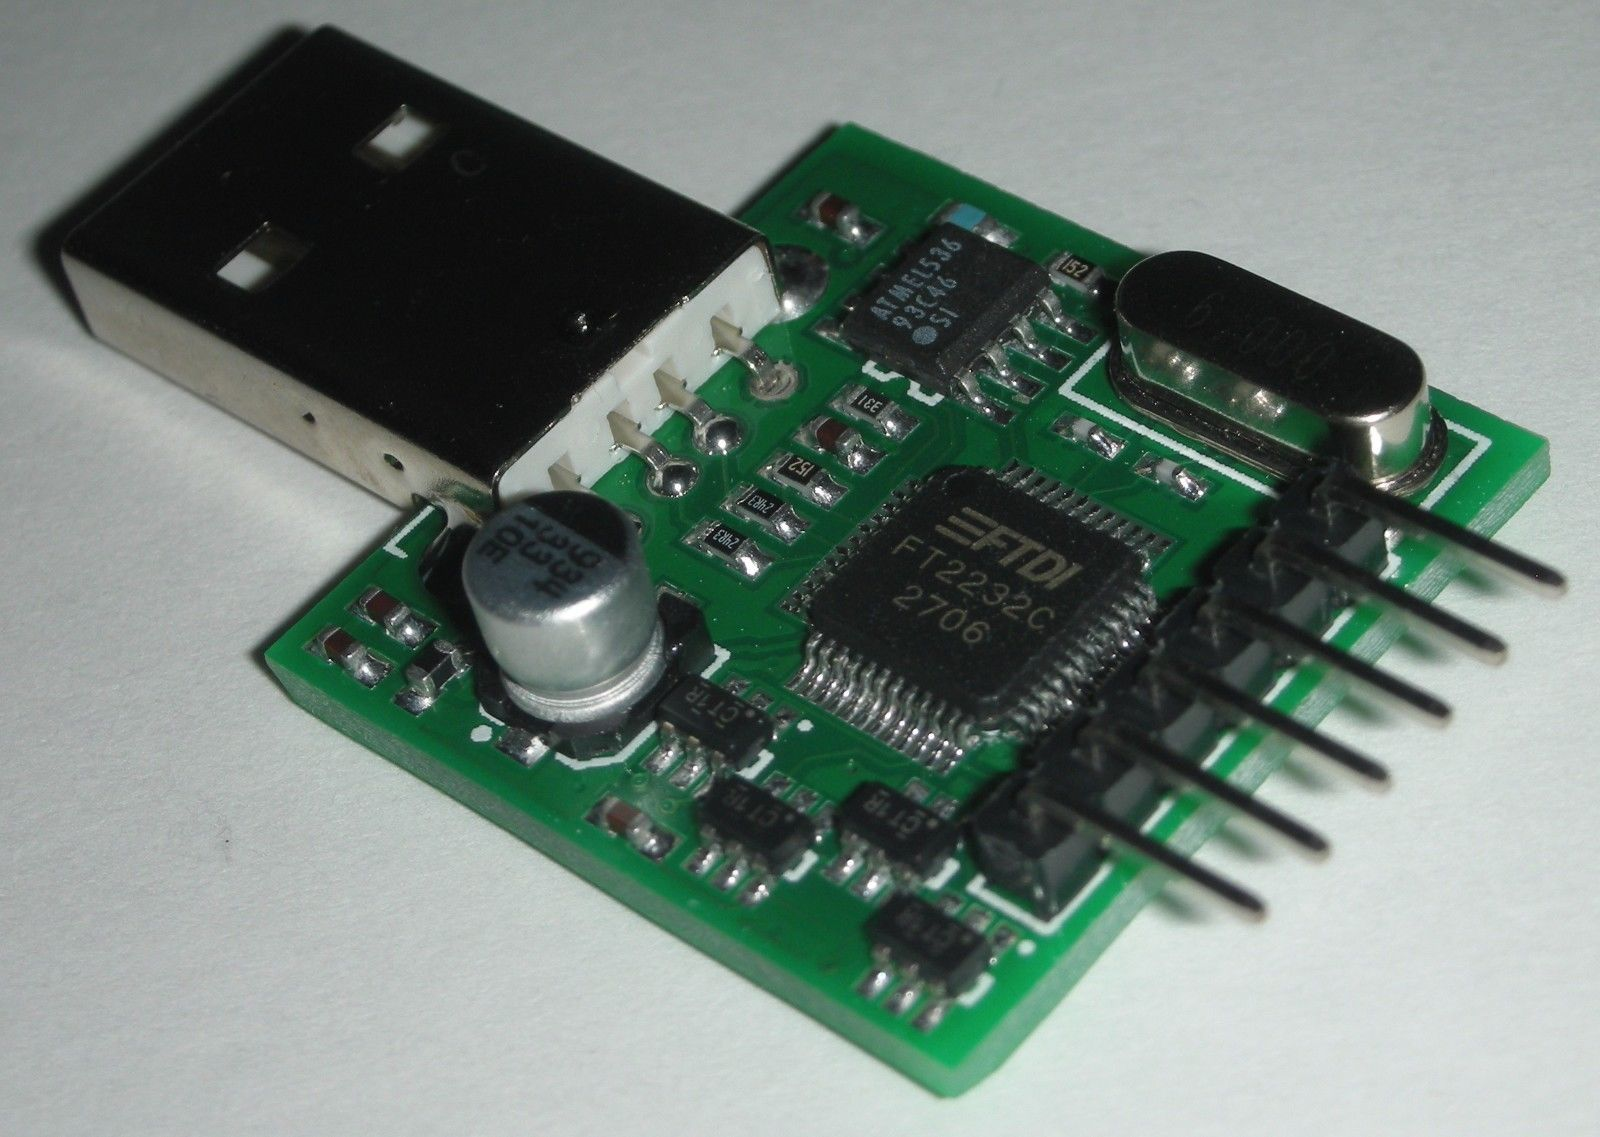
\includegraphics[width=\textwidth,height=\textheight,keepaspectratio]{images/JTAGAdapter.jpg}
		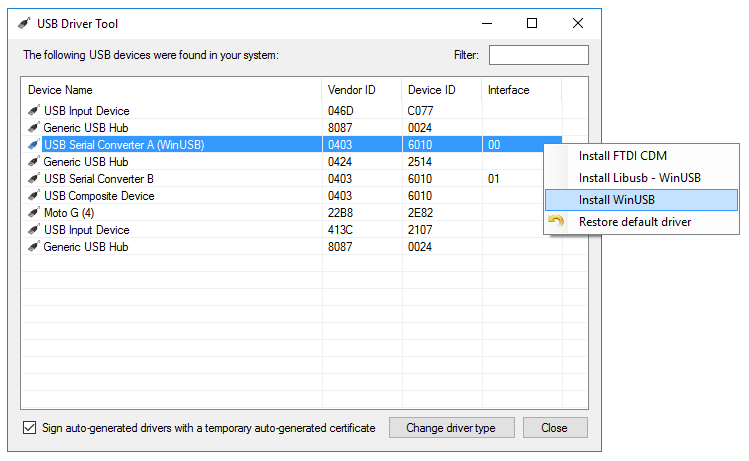
\includegraphics[width=12cm,keepaspectratio]{images/InstallWinUSBDriver.png}
	\caption{Installation des \textit{WinUSB} Treibers mit dem \textit{USB Driver Tool}}
	\label{fig:InstallWinUSBDriver}
\end{figure}


\section{OpenOCD CLI - Command Line Interface}
Das CLI (\textit{Command Line Interface}) ist eine einfache Methode um mit dem Debugger zu kommunizieren.
Sobald OpenOCD gestartet wurde, kann über den Port 4444, z.B. mit \textit{Putty}, auf dem \textit{Localhost} eine Telnet-Verbindung aufgebaut werden.
Der Befehl \texttt{''help''} listet alle zulässigen Befehle auf.

In den folgenden Kapiteln wird folgende Notation verwendet, um einen CLI-Befehl zu beschreiben:\\
(\texttt{CLI: Befehl})


\section{OpenOCD Konfiguration - Einleitung}
% TODO: zum starten siehe kapitel ...
% TODO: Files anhängen
% nicht einfach
% spezielle sprache jim-tcl
OpenOCD unterstützt eine Vielzahl von Adaptern und Targets (Prozessoren).
Beim Start muss die Software für die verwendete Hardware konfiguriert werden.
Die Konfiguration erfolgt mit Konfigurationsscripts (*.cfg) in der Scriptsprache \textit{Jim-Tcl}\footnote{http://jim.tcl.tk/index.html/doc/www/www/index.html}.
\textit{Jim-Tcl} ist eine abgespeckte Version von \textit{Tcl}\footnote{http://www.tcl.tk}.

Normalerweise werden die Scripts in die drei Gruppen \textit{interface, board} und \textit{target} aufgeteilt.
So kann einfach ein Script ausgewechselt werden, wenn man den gleichen Adapter aber einen anderen Prozessor verwenden will.
Im Pfad \texttt{openocd-0.10.0/scripts} befindet sich eine Sammlung von Konfigurationsscripts für Standardhardware.

Mit folgendem Befehl kann OpenOCD mit der passenden Konfiguration für das Zybo gestartet werden:\\
\texttt{openocd -f zybo-ftdi.cfg -f zybo.cfg}


\section{OpenOCD Konfiguration - Interface}
Die Interfacekonfiguration beschreibt hauptsächlich den verwendeten Adapter.
Da beim Zybo kein Adapter verwendet wird, sondern der aufgelötete FT2232, wird mit diesem Script der FTDI-Chip und dessen Anbindung an den Zynq konfiguriert.

Da ein FTDI-Chip als Interface verwendet wird, sollte ein passender Script unter \textit{openocd-0.10.0/scripts/ interface/ftdi/} zu finden sein.
Keiner der Scripts passt vom Namen her auf \textit{Zybo} oder \textit{FT2232}.
Eine Google Suche nach einem passenden Script war erfolgreicher.
Ein Github User mit dem Namen \textit{emard} hat folgenden Script in einem von seinen Repositories\footnote{https://github.com/f32c/f32c/blob/master/rtl/proj/xilinx/zybo/xram\_bram\_hdmi\_ise/zybo.ocd} gespeichert:

\textit{zybo-ftdi.ocd:}
\lstset{language=tcl}
\begin{lstlisting}[frame=single]
#
# ZYBO ft2232hq usbserial jtag
#

interface ftdi
ftdi_device_desc "Digilent Adept USB Device"
ftdi_vid_pid 0x0403 0x6010

ftdi_layout_init 0x3088 0x1f8b
#ftdi_layout_signal nTRST -data 0x1000 -oe 0x1000
# 0x2000 is reset
ftdi_layout_signal nSRST -data 0x3000 -oe 0x1000
# green MIO7 LED
ftdi_layout_signal LED -data 0x0010
#ftdi_layout_signal LED -data 0x1000

reset_config srst_pulls_trst

\end{lstlisting}

Zeile 5 bis 7 konfigurieren das Interface als ein Standard-FTDI-Interface.
Von OpenOCD werden neben dem FT2232 auch noch andere Chips unterstützt.
Zeile 7 definiert die \textit{Vendor} und \textit{Device-ID} des USB Devices.


\subsection{Resetverhalten}
Liest man aus einer unerlaubten Speicheradresse (\texttt{CLI: mdw 0x40000000}), dann hängt sich die Debug-Peripherie des Zynq auf.
Nach einem unerlaubten Speicherzugriff können auch keine erlaubten Speicherstellen mehr gelesen werden.
Beim Versuch erscheint die Fehlermeldung:\\
\texttt{Timeout waiting for cortex\_a\_exec\_optcode}.\\
Wahrscheinlich ist die \textit{CoreSight} Debug-Peripherie abgestürzt oder in einem undefinierten Zustand.
Aus diesem Grund bekommt OpenOCD keine Antwort vom Zynq, wenn versucht wird, eine Speicheradresse zu lesen.
Mit einem manuellen Powercycle vom Zybo kann die Hardware wieder zurückgesetzt werden.

Im Supportbereich der Xilinx Homepage\footnote{https://www.xilinx.com/support/answers/63871.html} ist eine mögliche Erklärung für dieses Verhalten zu finden.
In diesem Artikel wird beschrieben, dass die Fehlermeldung ''\textit{Invalid address - it can hang PS interconnect}'' erscheint, wenn mit dem XSDB (\textit{Xilinx System Debugger}) auf bestimmte Adressbereiche zugegriffen wird.
Die Vermutung liegt nahe, dass der XSDB merkt, wenn auf eine \textit{''Invalid address''} zugegriffen werden soll.
Dieser Befehl wird abgefangen und stattdessen wird die Fehlermeldung angezeigt, so dass der \textit{''PS interconnect''}, also der Bus innerhalb des Zynq, nicht abstürzen kann.
OpenOCD fängt einen solchen invaliden Zugriff nicht ab, was dann zum Absturz des \textit{''PS interconnect''} führt.
Da auch die Peripherie für den Debugger im Zynq von diesem \textit{Interconnect} abhängig ist, stürzt auch die Debug-Peripherie ab, sobald auf einen ungültigen Adressbereich zugegriffen wird.

Mit OpenOCD ist es grundsätzlich möglich, einen Reset automatisch durchzuführen.
Dabei wird zwischen einem SRST (\textit{System Reset}) und dem TRST (\textit{TAP Reset}) unterschieden.
% Dabei wird zwischen einen SRST (\textit{System Reset}) und dem \textit{TAP\footnote{Test Access Port} Reset} (TRST) unterschieden.
Der SRST führt einen Powercycle vom ganzen System durch, der TRST setzt mit einem JTAG-Befehl nur den TAP (\textit{Test Access Port}) zurück.

% TODO: warum memory location nicht erlaubt
Beim obigen Script ist aber das Resetverhalten nicht sauber definiert.
Mit dem Befehl \texttt{''CLI: reset halt''} sollte der FT2232 einen Reset des ganzen Zynq durchführen.
Der Befehl führt aber zur Fehlermeldung:\\
\texttt{
% ...\\
zynq.cpu0: how to reset?\\
% ...
}

Im OpenOCD User Manual\cite{bib:OpenOCDDoku} in \textit{''Kapitel 9: Reset Configuration''} ist beschrieben, wie das Resetverhalten konfiguriert werden kann.
Mit dem Script-Befehl \texttt{''reset\_config srst\_only''} wird der TAP Reset ignoriert.
Da jetzt nur noch der SRST und nicht mehr der TRST verwendet wird, kann das Problem auf den SRST begrenzt werden.

Wenn OpenOCD mit der neuen Konfiguration neu gestartet wird, scheint der Befehl \texttt{''CLI: reset halt''} zu funktionieren.
Wird vorher aber wieder auf eine ungültige Speicherstelle zugegriffen, dann erscheint beim Reset die Fehlermeldung:\\
\texttt{
% ...\\
Timeout waiting for dpm prepare\\
% ...\\
}\\
Das erneute Timeout legt die Vermutung nahe, dass der Zynq nicht ordentlich zurückgesetzt wurde.

Zeile 12 \texttt{''ftdi\_layout\_signal nSRST -data 0x3000 -oe 0x1000''} konfiguriert die I/O Pins des FT2232, welche für den System Reset verwendet werden.
Im elektrischen Schema des Zybos (siehe Anhang \ref{anhang:schemaZybo}) könnte man überprüfen, welche I/Os des FT2232 tatsächlich für den Reset verwendet werden.
Die Seite mit dem Schema für den FT2232, Seite 7, ist aber als einzige Seite im Schema nicht veröffentlicht worden.
Die korrekten I/O Pins lassen sich also nicht mit dem Schema ermitteln.

Im OpenOCD User Manual\cite{bib:OpenOCDDoku} wird der \texttt{''ftdi\_layout\_signal nSRST} genauer beschrieben.
Der Switch \textit{-data 0x3000} definiert alle relevanten Pins für den SRST und \textit{-oe 0x1000} konfiguriert alle Ausgänge.
In einem Versuch wurden diverse Kombinationen für die beiden Switches ausprobiert.
Keine Kombination mit nur einem Pin (z.B. \textit{-data 0x2000} mit \textit{-oe 0x2000}) hat funktioniert.
Es hat sich herausgestellt, dass die Kombination \textit{-data 0x3000} mit \textit{-oe 0x3000} tatsächlich einen System Reset ermöglicht.

Weil der Debugger direkt nach dem SRST versucht mit dem Zynq zu kommunizieren, tritt folgende Fehlermeldung auf:\\
\texttt{
...\\
Invalid ACK (7) in DAP response\\
JTAG-DP STICKY ERROR\\
...\\
}
Mit dem Kommando \texttt{''adapter\_nsrst\_delay 40''} wartet der Debugger nach dem SRST zusätzliche 40 Millisekunden.
Diese Wartezeit genügt, damit die FTDI-Interface wieder betriebsbereit ist, wenn der Debugger zu kommunizieren versucht.



\section{OpenOCD Konfiguration - Board}
Da beim Zybo der Adapter direkt auf dem Board ist, ist die Bordkonfiguration bereits im Konfigurationsscript für das Interface enthalten.

\section{OpenOCD Konfiguration - Target}
Für das Target, in diesem Fall der Zynq 7000 SOC, ist bereits ein Script unter \textit{openocd-0.10.0/scripts/ target/zynq\_7000.cfg} enthalten.
In diesem Script werden nicht nur beide Kerne des Prozessors definiert, sondern auch ein TAP für das FPGA.
Es ist also auch möglich, den FPGA mit dieser Toolchain zu laden.
% zynq_7000.cfg